\newpage

\section{Partie 1: Quelques opérations de base sur les signaux}

\subsection{Signal numérique de synthèse}

\subsubsection{Génération du signal}

Un signal sinusoïdal de fréquence \( f_0 \) est généré par la fonction suivante:

\[
x[n] = \sin\left(2\pi f_0 \frac{n}{f_e}\right)
\]

où \( f_e \) est la fréquence d’échantillonnage et \( N \) le nombre d’échantillons.

\begin{figure}[!h]
\centering
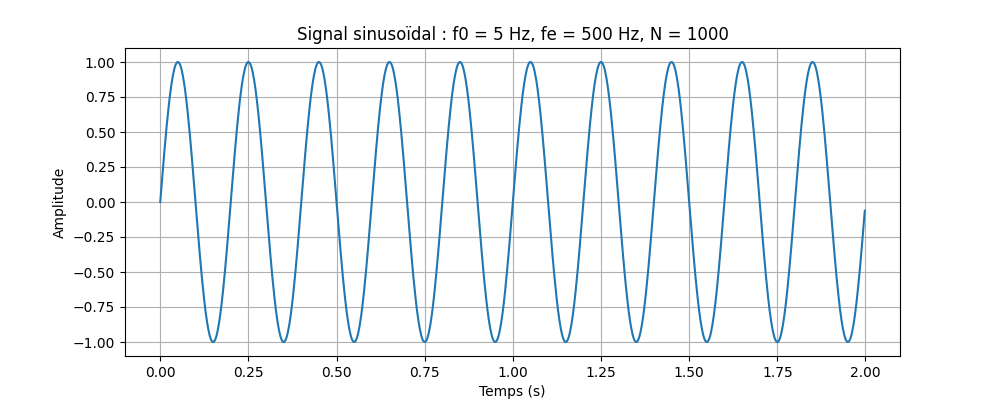
\includegraphics[width=17cm]{screenshots/signal_echantillone.png}
\caption{Signal sinusoïdal échantillonné}
\end{figure}

\subsubsection{Énergie et puissance}

L'énergie d’un signal discret \( x[n] \) est donnée par :

\[
E = \sum_{n=0}^{N-1} x[n]^2
\]

Et la puissance moyenne par :

\[
P = \frac{1}{N} \sum_{n=0}^{N-1} x[n]^2
\]

Considérons un signal sinusoïdal discret de la forme :
\[
x[n] = A \cdot \sin\left(2\pi f_0 \frac{n}{f_e} \right)
\]

La puissance moyenne théorique d’un signal périodique est calculée par la  formule:

\[
P = \lim_{N \to \infty} \frac{1}{N} \sum_{n=0}^{N-1} x[n]^2
\]

En utilisant l’identité trigonométrique :
\[
\sin^2(\theta) = \frac{1 - \cos(2\theta)}{2}
\]
on obtient :
\[
x[n]^2 = A^2 \cdot \frac{1 - \cos\left(4\pi f_0 \frac{n}{f_e} \right)}{2}
\]

Ainsi, la puissance devient :
\[
P = \lim_{N \to \infty} \frac{1}{N} \sum_{n=0}^{N-1} A^2 \cdot \frac{1 - \cos\left(4\pi f_0 \frac{n}{f_e} \right)}{2}
= \lim_{N \to \infty}  \frac{A^2}{2} - \frac{A^2}{2N} \sum_{n=0}^{N-1} \cos\left(4\pi f_0 \frac{n}{f_e} \right)
= \frac{A^2}{2}
\] 

Donc dans notre cas la puissance moyenne théorique est égale à 0.5.

Pour la puissance moyenne calculée numériquement pour le signal échantillonné on a la méme formule mais sans la limite:

\[
P = \frac{A^2}{2} - \frac{A^2}{2N} \sum_{n=0}^{N-1} \cos\left(4\pi f_0 \frac{n}{f_e} \right)
\] 

\textbf{Cas idéal :} si $N$ est un multiple entier de la période du signal (i.e., $N$ couvre un nombre entier de périodes), alors la somme des cosinus s’annule :
\[
\sum_{n=0}^{N-1} \cos\left(4\pi f_0 t \right) = 0 \quad \Rightarrow \quad P = \frac{A^2}{2}
\]

\textbf{Cas général :} si $N$ n’est pas un multiple exact de la période, la somme ne s’annule pas et on observe une légère déviation de la puissance par rapport à $\frac{A^2}{2}$. Cela est dû au fait que le signal est tronqué entre deux points non symétriques.\\

En variant N on trouve plusieurs valeurs de la puissance moyenne qui restent proches de la valeur théorique:

\begin{figure}[!h]
\centering
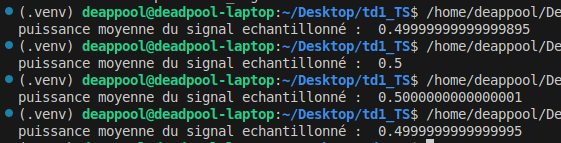
\includegraphics[width=15cm]{screenshots/puissance_et_energie.png}
\caption{Énergie et puissance du signal}
\end{figure}

\subsubsection{Quantification}

Le processus de quantification consiste à projeter les valeurs continues du signal sur un ensemble discret de niveaux. Une erreur courante est de laisser les bornes \([-1, 1]\) incluses, ce qui n’est pas conforme à une quantification uniforme centrée autour de zéro. Le code corrigé est le suivant :

\begin{lstlisting}[language=python]
def quantifier(signal, N_bits):
    levels = 2 ** N_bits
    step = 2 / levels  # [-1 + step/2, 1 - step/2]
    quantized_signal = np.clip(np.round(signal / step) * step, -1 + step, 1 - step)
    return quantized_signal
\end{lstlisting}

\begin{figure}[!h]
\centering
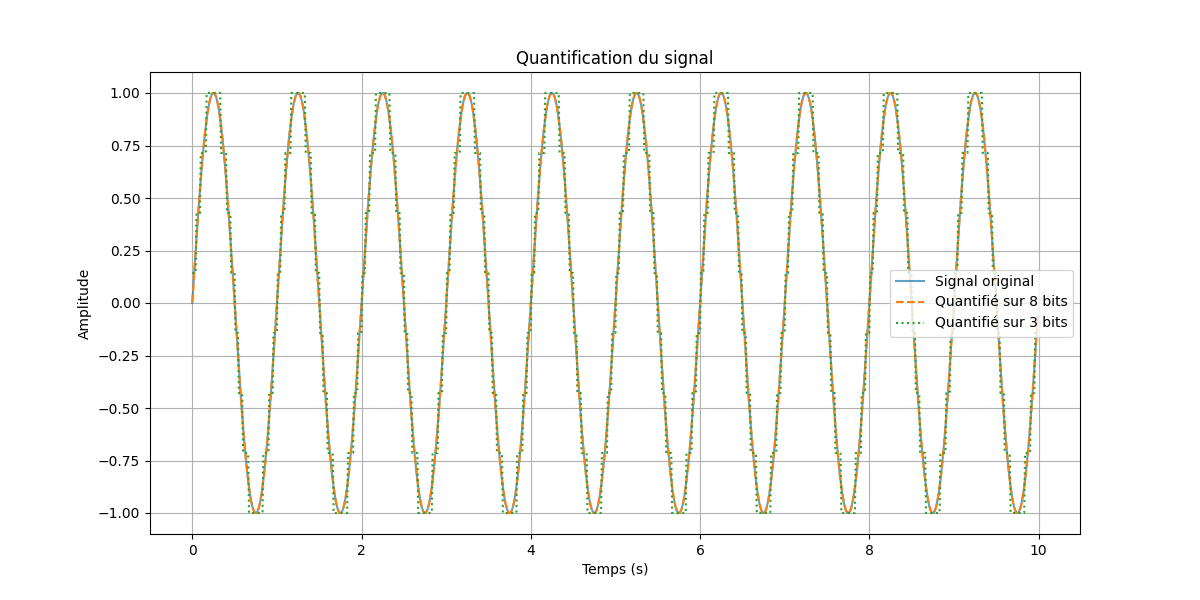
\includegraphics[width=17cm]{screenshots/Quantification.png}
\caption{Quantification du signal à 3 et 8 bits}
\end{figure}

Le signal à 8 bits épouse mieux la forme continue du signal d’origine. À 3 bits, les marches sont visibles.

\textbf{SNR (Signal-to-Noise Ratio)} :

\[
\text{SNR} = 10 \log_{10} \left(\frac{E_{\text{signal}}}{E_{\text{bruit}}} \right)
\]

Des valeurs corrigées et réalistes sont obtenues :

\begin{itemize}
    \item \( SNR_{8} \approx 49.7\, \text{dB} \)
    \item \( SNR_{3} \approx 19.6\, \text{dB} \)
\end{itemize}

\begin{figure}[!h]
\centering
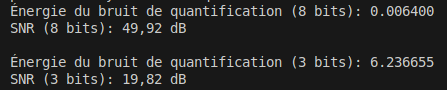
\includegraphics{screenshots/snr_quantification.png}
\caption{SNR pour chaque niveau de quantification}
\end{figure}

\subsection{Signal audio}

\subsubsection{Enregistrement}

Les mots « Bonjour » et « ChatGpt » ont été enregistrés via Audacity. 

\subsubsection{Restitution à différentes fréquences}

L’audio est lu à \( f_e \), \( 2 f_e \) et \( \frac{f_e}{2} \). 

\textbf{Effets observés} :

\begin{itemize}
    \item \textbf{Durée :} doubler la fréquence de restitution divise la durée par deux (voix accélérée), tandis que la diviser par deux double la durée (voix ralentie).
    \item \textbf{Hauteur :} multiplier la fréquence de restitution rend la voix plus aiguë (fréquences doublées), la diminuer la rend plus grave (fréquences divisées).
    \item \textbf{Applications :} cette manipulation illustre le principe de transposition spectrale et d’étirement temporel.
\end{itemize}

\subsubsection{Quantification du signal audio}

\begin{itemize}
    \item À 3 bits : le son devient rugueux et très bruité, fortement altéré.
    \item À 8 bits : la voix reste compréhensible mais moins naturelle.
    \item À 16 bits (original) : qualité fidèle.
\end{itemize}

\subsubsection{Extraction et séparation de mots}

Après repérage visuel, les deux mots ont été extraits via tranches temporelles, puis enregistrés :

\begin{lstlisting}[language=python]
sf.write("mot1.wav", mot1, fe)
sf.write("mot2.wav", mot2, fe)
\end{lstlisting}

\begin{figure}[h]
\centering
\begin{subfigure}[b]{0.45\textwidth}
    \centering
    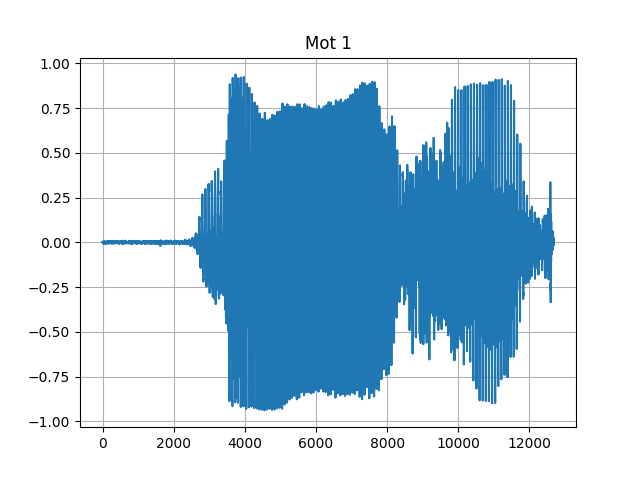
\includegraphics[width=9cm]{screenshots/mot1_graphe.png}
    \caption{Mot 1: "Bonjour"}
\end{subfigure}
\hfill
\begin{subfigure}[b]{0.45\textwidth}
    \centering
    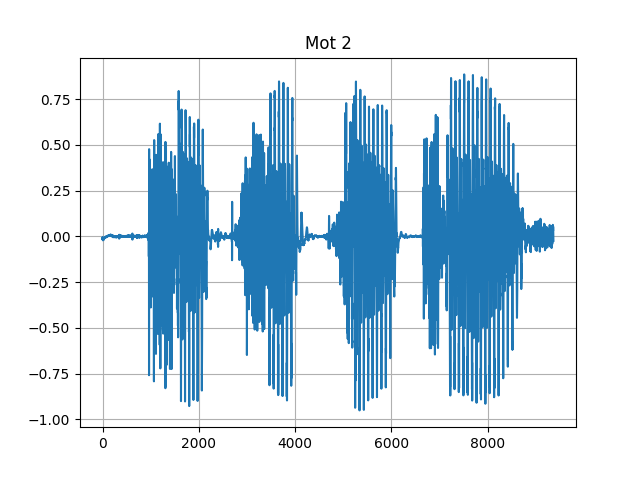
\includegraphics[width=9cm]{screenshots/mot2_graphe.png}
    \caption{Mot 2: "ChatGpt"}
\end{subfigure}
\caption{Séparation des mots dans le signal audio}
\end{figure}


\subsubsection{Extraction de mots}

Aprés avoir identifié l'intervalle de temps pour chaque mot dans le signal enregistré on utilise ce code pour séparer les deux mots:
\begin{lstlisting}[language=python]
n1 = int(0.3 * fe)     #0.3s 
n2   = int(2.3 * fe)   #2.3s 
n3 = int(4 * fe)       #4s 

mot1 = y[n1:n2]
mot2 = y[n2+1:n3]

print("Mot 1 :")
sd.play(mot1, fe)
sd.wait()

print("Mot 2 :")
sd.play(mot2, fe)
sd.wait()
\end{lstlisting}

\begin{figure}[h]
    \centering
    \begin{subfigure}[b]{0.45\textwidth}
        \centering
        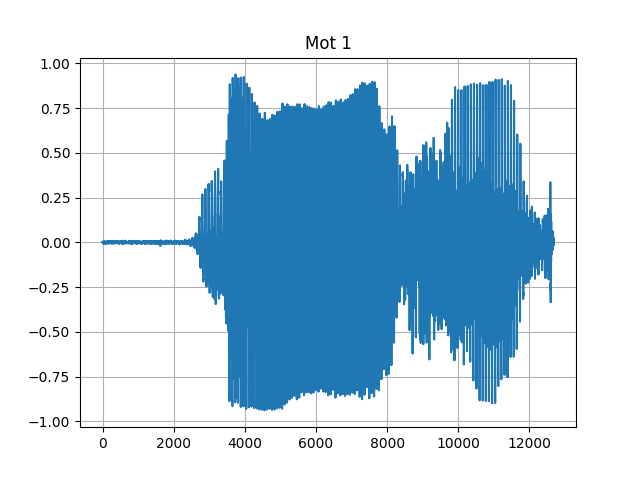
\includegraphics[width=9cm]{screenshots/mot1_graphe.png}
        \caption{Mot 1}
        \label{fig:mot1}
    \end{subfigure}
    \hfill
    \begin{subfigure}[b]{0.45\textwidth}
        \centering
        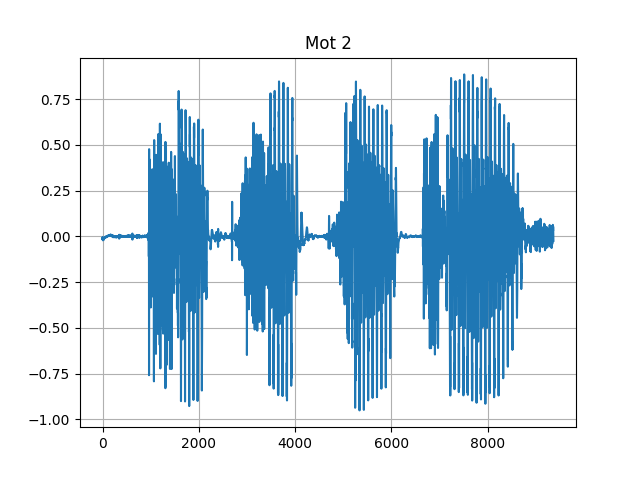
\includegraphics[width=9cm]{screenshots/mot2_graphe.png}
        \caption{Mot 2}
        \label{fig:mot2}
    \end{subfigure}
    \caption{Séparation des deux mots}
    \label{fig:Séparation des deux mots}
\end{figure}

Puis on enregistre les deux mots séparément dans des fichiers .wav :
\begin{lstlisting}[language=python]
    sf.write("mot1.wav", mot1, fe)
    sf.write("mot2.wav", mot2, fe)
\end{lstlisting}